%%% Thesis Introduction --------------------------------------------------
\chapter{Introduction}
\ifpdf
    \graphicspath{{Chapters/Introduction/IntroductionFigs/PNG/}{Chapters/Introduction/IntroductionFigs/PDF/}{Chapters/Introduction/IntroductionFigs/}}
\else
    \graphicspath{{Chapters/Introduction/IntroductionFigs/EPS/}{Chapters/Introduction/IntroductionFigs/}}
\fi

\begin{figure}[htb]
   	\centering
   	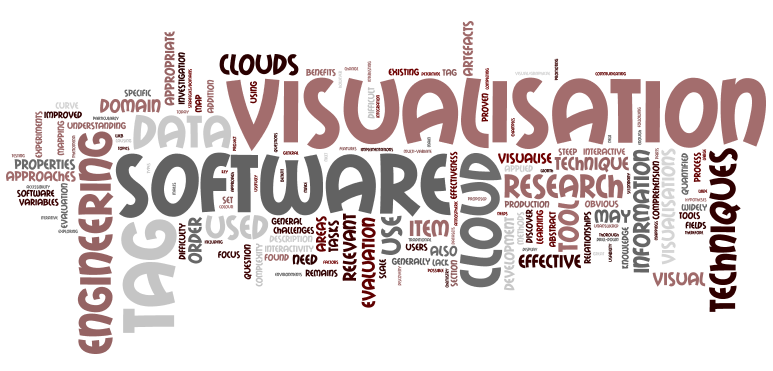
\includegraphics[scale=0.55]{tagcloud.png}
	\label{fig:tagcloud}	
\end{figure}

\section{Motivation}

Visualisations, or graphical representations of data, are thought to be an effective method of communicating information and are used everywhere in our daily lives, from weather maps to road signs. Visualisations based on an underlying physical model are heavily used in scientific fields such as physics, chemistry, medicine and atmospheric sciences to increase understanding and to confirm or reject hypotheses. In other research areas, information visualisation is used to discover interesting phenomena in unknown and abstract data. Visualisation has long been used as a way to deal with large datasets --- the more data in a dataset, the greater the need and the greater the pay-off for visualisation. Ultimately all visualisation is about ``things'', their detailed properties and their relationships. In tag clouds, ``things'' are displayed through tags, properties are displayed through various field values, and relationships are shown through the tag order, layout, or through explicit connections.

Software is a domain where visualisation is sorely needed. Modern software systems are notoriously large and complex --- this complexity makes them difficult to understand, develop and maintain, causing costly IT project failure, and budget or timeline blow-outs. We clearly need more effective methods of promoting comprehension of software in addition to the modern software development approaches such as iterative development and automated unit testing. Approaches exist to visualise abstract software artefact properties such as algorithms, metrics, process data and relationships. However, despite the seemingly obvious benefits of using visualisation and the existing research efforts surrounding the software visualisation domain, it is not widely practised or integrated into mainstream development environments \citep{reiss05}.

The question of why this is the case remains largely unanswered, but some possibilities include; a) existing models and techniques having a steep learning curve, or the concepts are difficult to quickly grasp, b) visualisations not scaling well to the demands of a software engineering dataset, and c) techniques not being adequately and demonstrably proven to have a benefit, and therefore not potentially being worth the effort of integration into a workflow. Although a wide range of visualisations have been proposed for the software engineering domain, there remains the need to explore new techniques, particularly those with a low level of conceptual complexity, and for the effectiveness of visualisation tools and techniques to be quantified.

\section{Research questions}

It may be that the difficulty of software comprehension could be improved with effective use of visualisation techniques, but these techniques are not widely applied in industry. A variety of factors including the steep learning curve of visualisation techniques and a general lack of quantified effectiveness potentially contribute to this.

Enter tag clouds, a simple and highly recognisable visualisation commonplace on the web today. Some of the main benefits of using tag clouds as an information visualisation technique are their accessibility and visual interestingness, and the fact they have a set of visual properties (such as font size and text colour) that make it possible to map to data variables. Labels and textual identifiers are an intrinsic part of the visual encoding, enabling users to determine key information without the need to navigate around or drill-down. As an effective visualisation, tag clouds suffer from some drawbacks --- these are generally related to the limited interactivity provided in traditional implementations, such as the inability to change order or layouts on the fly. This lack of interactivity causes great difficulty in the process of exploration of data.  With the addition of such features generally found in a visualisation tool, can the tag cloud metaphor be extended to successfully visualise multi-variate data such as that found in software engineering? 

The research reported in this thesis takes the tag cloud visualisation technique and applies it to the software engineering domain. The primary research question pursued was to discover if visualisation of relevant software engineering data artefacts with a tag cloud could promote a greater understanding of a software system, in particular if it would assist users in completing specific types of tasks. This was divided broadly into the following secondary areas of research:

\pagebreak

\paragraph{Design choices for an interactive tag cloud tool}
\begin{itemize} 
\item defining visual properties that may influence perception in tag clouds
\item selecting visual properties that are appropriate for data mapping 
\item how to appropriately use characteristics of visual properties
\item challenges and special needs in a software engineering dataset
\item task types to enable data exploration in a tag cloud
\item applying the resulting design considerations to an interactive tool
\end{itemize} 

\paragraph{Previous evaluations in tag cloud research}
\begin{itemize}
\item using prior tag cloud evaluations to shape our research focus and build an overview of tag cloud knowledge in general
\item the extent to which each topic has been evaluated
\item evaluation approaches and methods, fields and domains
\end{itemize} 

\paragraph{Evaluation of our interactive tag cloud tool}
\begin{itemize}
\item evaluation strategies and methodologies which match our research goals
\item how to evaluate our tool in as broader manner as possible
\item discovering whether our tool is usable and comprehensible
\item discovering whether the tool is easy to learn
\item investigating if the enhanced tag cloud techniques provided in our prototype provide an improvement in user performance
\item investigating if the tool can be used to discover knowledge about an unknown software engineering dataset, with a minimum of training
\end{itemize} 


\section{Approach}

Using the analysis of design considerations and task types detailed in Chapter~\ref{chap:tagcloud}, we extended and altered existing software to produce a novel interactive tag cloud visualisation tool. This tool was designed to cope with the specific challenges of software engineering datasets using appropriate visual mappings available in tag clouds to render the data, and is introduced in Chapter~\ref{chap:taggle}.

It can be a challenging task to evaluate information visualisation techniques because of the difficulties in capturing and quantifying the data exploration process. We embarked on a systematic mapping study (Chapter~\ref{chap:strateval}) of previous research evaluating the tag cloud technique or interactive tools that included tag cloud visualisation. Topics, fields or domains that had not been extensively researched, and approaches and methods which had been used for evaluation were identified. This provided a big picture view of what was known about tag clouds, and helped us plan and focus our overall evaluation strategy. An evaluation map (Chapter~\ref{chap:eval}) was created to plan a broad-base investigation of points of relevance for both the tag cloud technique and our interactive tool, with selection of experimental methodology based on research goals.

As part of our overall evaluation strategy, a heuristic evaluation by domain experts was performed (Chapter~\ref{chap:heuristiceval}). Subjective user feedback was elicited to clarify research questions around the comprehensibility of the visualisation technique and data mapping process, as well as assessing the system usability. This evaluation generated various prototype design refinements and satisfied us that the tool was mature enough for use in more detailed experimentation.

Following the heuristic evaluation, three experiments were completed in order to explore the potentials and limitations of the interactive tag cloud visualisation tool. In order to obtain a broad evaluation of relevant parts of the tool, these experiments were conducted in both areas of \emph{visualisation use} (the tag cloud technique) and \emph{data analysis process} (a whole-tool approach focused on the knowledge discovery process). Properties of the enhanced tag cloud features utilised in the interactive system were investigated in two experiments using eye-tracking technology (Chapter~\ref{chap:exp1} and Chapter~\ref{chap:exp2}) to discover if improvements could be made in user performance for visual search tasks.  The results of the \emph{visualisation use} experiments have wider implications than just for our interactive tool alone, and are relevant for designers of tag cloud visualisations. To evaluate the tool in a more holistic fashion, an empirical user study was conducted to examine data exploration and knowledge discovery support for software engineering data in our interactive system. The extent to which the system was efficient in facilitating knowledge discovery was gauged through analysis of domain appropriate benchmark task completion rates. Eye-gaze data was also collected for all experiments and analysed for user visual search patterns in tag clouds, and to study usage of various areas of interest within the interactive interface. 

\section{Contributions}

The contributions of this thesis can be categorised into four areas: 

\begin{itemize}
	\item Design considerations for an interactive tag cloud visualisation system. We analysed the challenges in visualising multi-variate data, and the capabilities of tag clouds --- in particular the effects on user perception for available visual properties according to various design principles, guidelines, and current research. We defined the appropriateness of visual variables for data mapping, and task types that should be supported in order to enable data exploration.
	\item Systematic mapping study of existing tag cloud evaluation research. This provided an overview of existing evaluations of the tag cloud visualisation and tools which incorporated the technique. There was a strong prevalence in the research to focus on web and user generated data domains, using a limited range of evaluation approaches.
	\item The design and evaluation of a novel tag cloud visualisation system.  
	\begin{enumerate}[(a)]
		\item `Taggle' system created in accordance with the design considerations (through extensions and alterations to existing software) in order to explore multi-variate data such as software quality assurance measurements. 
		\item Subsequent design refinements were necessary following a heuristic evaluation by domain experts, where the system was evaluated for usability and appropriateness of exploration of multi-variate data. The study revealed the tag cloud technique of contrasting visual font properties mapped to data fields was felt to be instinctively comprehensible, but the amount of information that could be inferred was greatly dependent on the software's support for selection of appropriate mappings.  
		\item The system's support for data exploration and knowledge discovery was evaluated through an empirical user study. Results were encouraging, showing `Taggle' could be used with minimal training to discover relevant information about an unknown software engineering dataset. Eye-gaze data showed participants who successfully completed tasks highly utilised the data summary panel and rich interactive features such as mapping multiple visual properties to data fields, and static and dynamic filtering.
      \end{enumerate}
	\item The evaluation of enhanced tag cloud features utilised in the interactive system through  user experiments. The results of these experiments have implications for designers of tag cloud visualisations, and provide insight into tag cloud visual search patterns.
	\begin{enumerate}[(a)] 
		\item \emph{Tag background colour} Results indicated usage of tag background colour as a data variable field can produce faster visual search response time than font colour in a tag cloud, when the target tag is small. 
		\item \emph{Dual data mappings} Dual mappings of font size and colour can produce faster visual search response times than singular mappings of font size or colour alone.
		\item \emph{Visual search patterns} Previous eye-tracking studies have identified user serial scanning and chaotic search methods within tag clouds.  Our eye-tracking data analysis showed the introduction of a visual property hint when performing a search task, can alter the search strategy to the eye-scan path focusing on tags with the target mapping (efficient feature search). When task complexity is increased, users generally employed combination visual search methods in a tag cloud, switching between visual feature search, serial scanning and chaotic search methods.
       \end{enumerate}
\end{itemize}

\section{Outline}

This thesis presents the following relevant information:

\begin{description}
	\item[Chapter~\ref{chap:background} \emph{Background}] Describing current software engineering practices, how they attempt to address quality issues and manage the manifold complexities existing in today's software systems. Basics in visualisation and software visualisation. Introduction to the tag cloud, benefits of usage, and limitations of currently available software engineering tools which incorporate tag clouds. 
	\item[Chapter~\ref{chap:tagcloud} \emph{Design considerations for interactive tag cloud visualisation}] Discussion of visual variables in a tag cloud which may be manipulated to represent data variables. Challenges in software visualisation and task types that represent meaningful ways users may interact with software data.
	\item[Chapter~\ref{chap:taggle} \emph{Taggle: A tag cloud visualisation tool}] Presentation of the tag cloud visualisation tool Taggle implemented according the the design considerations. Description of the data model and transformations, the visual encoding and mapping selection. Examples of how to use the tool to complete the software engineering tasks outlined in the previous chapter.
	\item[Chapter~\ref{chap:strateval} \emph{Systematic mapping study for tag cloud research}] Strategies that can be employed when evaluating an information visualisation tool. Description of a systematic mapping study performed to identify topics, fields or domains where tag cloud visualisation tools have been evaluated. Discovering what evaluation approaches and methods were used. 
	\item[Chapter~\ref{chap:eval} \emph{Evaluation strategy for Taggle}] Based on the outcomes of the systematic study, this chapter details the creation of an evaluation map outlining potential areas where Taggle could be evaluated along with sample methodologies. This was used to strategically plan a series of evaluations covering a broad base of relevant topics. Generation of experimental datasets and how the eye-tracking experimentation was conducted is also discussed.
	\item[Chapter~\ref{chap:heuristiceval} \emph{Heuristic evaluation of Taggle}] Description of a heuristic evaluation performed to elicit user feedback into the general usability of the tool, and to clarify research questions pertinent to the future experimentation as well as checking the tool was sufficiently mature to use in experimentation. Results and adaptations resulting from the evaluation are presented.
	\item[Chapter~\ref{chap:exp1} \emph{Experiment one: tag colour placement}] Description of an eye-tracking experiment performed to examine the specifics of the tag cloud technique used in Taggle --- specifically to ascertain how altering tag colour placement between font or tag background affected user performance for search tasks. Experiment design, procedure, results including eye-tracking and statistical analyses, and conclusions are presented.
	\item[Chapter~\ref{chap:exp2} \emph{Experiment two: dual mappings}] Description of an eye-tracking experiment performed to examine the specifics of the tag cloud technique used in Taggle --- specifically to ascertain how mapping a data variable to size or colour, compared to mapping a data variable to size and colour together, affected user performance for search tasks. Experiment design, procedure, results including eye-tracking and statistical analyses, and conclusions are presented.
	\item[Chapter~\ref{chap:exp3} \emph{Experiment three: knowledge discovery}] Description of an eye-tracking experiment performed to examine data exploration and knowledge discovery support in Taggle --- specifically to ascertain if and how Taggle supported the discovery of relevant software engineering information and if the tool was sufficiently easy to learn to complete the tasks with minimal training. Experiment design, procedure, results including eye-tracking and statistical analyses, and conclusions are presented.
	\item[Chapter~\ref{chap:conclusions} \emph{Conclusions}] Review of thesis contributions. Future work and limitations of the research are discussed.
	\item[Chapter~\ref{appendx:d} \emph{Publications}] Articles published as a result of this research.
\end{description}

%%% ----------------------------------------------------------------------


%%% Local Variables: 
%%% mode: latex
%%% TeX-master: "../thesis"
%%% End: 
